\documentclass[usepdftitle=false]{beamer}
\directlua{pdf.setminorversion(7)}

\usetheme[secheader]{Boadilla}
\usefonttheme{professionalfonts}
\setbeamertemplate{navigation symbols}{}

%
% Packages
%

\usepackage{fontspec}%
\usepackage[english]{babel}%
\usepackage[babel, final]{microtype}%

\usepackage{mathtools}%
\usepackage{amsthm}%
\usepackage{stmaryrd}%
\usepackage[ruled, longend]{algorithm2e}%
\usepackage{prftree}%
\usepackage{unicode-math}%

\usepackage{fancyvrb}%
\usepackage[newfloat]{minted}%

\usepackage{booktabs}%
\usepackage{graphicx}%
\usepackage[compatibility=false]{caption}%
\usepackage{subcaption}%

\usepackage{tikz}%
\usepackage{pgfplots}%
\usepackage{pgfplotstable}%

\usepackage[strict, autopunct]{csquotes}%
\usepackage[hyperref, citestyle=numeric-comp, backend=biber,%
maxcitenames=2, giveninits, isbn=false, url=false, doi=false]%
{biblatex}%

\usepackage{siunitx}%
\usepackage{nth}

\usepackage[shortcuts]{extdash}%

%
% Setup
%

\addbibresource{../Bibliography.bib}%
\unimathsetup{%
  math-style=ISO,%
  bold-style=ISO%
}%
\mathtoolsset{
  mathic%
}%
\graphicspath{{Figures/}{../}}%
\sisetup{%
  detect-all,%
  detect-display-math,%
  binary-units%
}%
\hypersetup{%
  unicode,
  pdfinfo={%
    Title={Introduction to Word Vectors},%
    Subject={Pattern Recognition},%
    Author={Dario Gjorgjevski},%
    Keywords={Deep Learning, Neural Networks, Distributed Representations}%
  }
}%
\pgfplotsset{compat=newest}%
\usetikzlibrary{patterns, fit, positioning, calc, shapes.arrows}%

\theoremstyle{definition}
\newtheorem{assumption}{Assumption}

%
% Commands
%

% Notation from linear algebra
\AtBeginDocument{%
  \renewcommand*{\vec}{\symbf}%
  \newcommand*{\mat}{\symbf}%
  \newcommand*{\trans}{\top}%
}%
\DeclareMathOperator{\rank}{rank}%
\DeclareMathOperator{\lspan}{span}%
\DeclareMathOperator{\supp}{supp}%
\DeclarePairedDelimiter{\basis}{\langle}{\rangle}%
\newcommand*{\M}{\ensuremath{\mathcal{M}}}%
\newcommand*{\GL}{\ensuremath{\mathsf{GL}}}%

% Notation from probability and statistics
\DeclareMathOperator{\E}{\mathbb{E}}%
\DeclareMathOperator{\var}{var}%
\DeclareMathOperator{\cov}{cov}%

% Asymptotic notation
\newcommand*{\BigOh}{\mathcal{O}}%

% Iverson bracket
\DeclarePairedDelimiter{\Iverson}{\llbracket}{\rrbracket}%

% Miscellaneous notation
\newcommand*{\ins}{\mathsf{(in)}}
\newcommand*{\outs}{\mathsf{(out)}}
\newcommand*{\negs}{\mathsf{(neg)}}

\DeclareMathOperator{\Left}{left}

%
% Title
%

\title{Introduction to Word Vectors}%
\subtitle{Learning Word Vectors Using \Verb+word2vec+ and Reasoning
  With Them}%
\author[Dario Gj.]{%
  Dario Gjorgjevski\inst{1}\\%
  \href{mailto:gjorgjevski.dario@students.finki.ukim.mk}%
  {\nolinkurl{gjorgjevski.dario@students.finki.ukim.mk}}%
}%
\institute[FCSE]{%
  \inst{1}Faculty of Computer Science and Engineering\\%
  Ss.\ Cyril and Methodius University in Skopje%
}%
\date{January 31, 2017}%

%
% Logo
%

% \logo{
\includegraphics[height=0.66cm]{Logo.png}}

%
% Table of contents
%

\AtBeginSection[]{%
  \begin{frame}{Contents}
    \tableofcontents[currentsection, hideothersubsections]
  \end{frame}
}


%
% Document
%

\begin{document}

\begin{frame}[plain, noframenumbering]
  \titlepage%
\end{frame}

\section{Motivation}

\subsection{Language Models}

\begin{frame}{What Is a Language Model?}
  \begin{definition}[Language Model]
    A \emph{language model} is a probability distribution over word
    sequences.  More formally, given a word sequence
    \(w_1, \ldots, w_m\), the language model assigns a probability
    \[
      p(w_1, \ldots, w_m)
    \]
    to the whole sequence.
  \end{definition}
  Until recently, the most widely used language model was the
  \emph{\(n\)\=/gram model}, which assumes an a Markov property of
  order \(n\).
\end{frame}

\begin{frame}{\(n\)\=/Gram Model}{Concept}
  In an \(n\)\=/gram model, the probability \(p(w_1, \ldots, w_m)\) is
  approximated as
  \begin{align*}
    p(w_1, \ldots, w_m) &= \prod_{i = 1}^{m} p(w_i \mid w_1, \ldots, w_{i - 1})\\
                        &\approx \prod_{i = 1}^{m} p(w_i \mid w_{i - (n - 1)}, \ldots, w_{i - 1})\text.
  \end{align*}
  \begin{itemize}
  \item The conditional probabilities can be calculated by counting;
    \alert{however},
  \item \emph{Smoothing} is required for unseen \(n\)\=/grams.
  \end{itemize}
\end{frame}

\begin{frame}{\(n\)\=/Gram Model}{Issues}
  \begin{itemize}
  \item As the \(n\)\=/gram model is trained on larger and larger
    texts, the vocabulary size increases as \(K n^{\beta}\) with
    \(10 \le K \le 100\) and \(0.4 \le \beta \le 0.6\)
    (\structure{\emph{Heaps' law}}).
  \item As the vocabulary size increases, the number of possible
    sequences of words increases exponentially \(\implies\) data
    sparsity problems.
  \item Ultimately, we are not sure how a word is to be even
    represented, and the \(n\)\=/gram model does not provide us with
    any clues toward that direction.
  \end{itemize}
\end{frame}

\subsection{Word Vectors}

\begin{frame}{Localist Representations}
  These representations are also called \emph{one\-/hot}.  They
  dedicate one unit to each word.
  \begin{itemize}
  \item Easy to understand.
  \item Easy to code by hand.
    \begin{itemize}
    \item Have been used as inputs to machine learning algorithms, especially
      neural networks.
    \end{itemize}
  \item Easy to learn.
    \begin{itemize}
    \item It is what mixture models (e.g., hidden Markov models) do.
    \end{itemize}
  \item Easy to associate with other representations or responses.
  \end{itemize}
  \alert{However}, they are terribly inefficient when the data has
  componential structure\--- and language does.
\end{frame}

\begin{frame}{Localist Representations}{Issues}
  In vector space terms, these are vectors with one \(1\) and lots of
  \(0\)s:
  \[
    \begin{bmatrix}
      \cdots & 0 & 0 & 1 & 0 & 0 & \cdots
    \end{bmatrix}\text.
  \]
  \begin{itemize}
  \item These vectors are \emph{extremely} sparse.
  \item They do not encode encode similarities whatsoever, i.e.,
    \[
      \forall i \ne j\ldotp \vec{w}_i \wedge \vec{w}_j = \vec{0}\text,
    \]
    even if \(\vec{w}_i\) and \(\vec{w}_j\) are semantically similar.
  \end{itemize}
\end{frame}

\begin{frame}{Distributional Representations}
  A lot of information can be obtained by representing a word by means
  of its neighbors.
  \begin{displayquote}[J.~R.~Firth]
    \structure{You shall know a word by the company it keeps.}
  \end{displayquote}
  How do we learn distributional representations?
  \begin{itemize}
  \item Directly, using co\=/occurrence matrices; or
  \item As a side\-/effect by training neural networks to predict
    either the word given its context, or the context given a word
    (\emph{continuous space language models}).
  \end{itemize}
\end{frame}

\section{Learning Word Vectors}

\subsection{Learning Context by Counting}

\begin{frame}{Co-Occurrence Matrices}
  \begin{definition}[Co-Occurrence Matrix]
    Let \(\{w_1, w_2, \ldots, w_V\}\) be the vocabulary.  A
    \emph{co\=/occurrence matrix} is a \(V \times V\) matrix which
    counts how many times a pair of words \((w_i, w_j)\) appear
    together in some context.
  \end{definition}
  \begin{itemize}
  \item Very straightforward solution.
  \item Can learn either:
    \begin{itemize}
    \item General topics by considering full documents as contexts; or
    \item Syntactic and semantic information by using a window
      context.
    \end{itemize}
  \end{itemize}
  The context is usually taken to be a window of size \(k\).
\end{frame}

\begin{frame}{Co-Occurrence matrices}{Issues}
  \begin{itemize}
  \item Dimension increases quadratically with \(V\) \(\implies\) huge
    storage requirements, sparsity issues in classifiers.
  \item Models are less robust because of sparsity issues.
  \item Low-dimensional vectors can be obtained by SVD\@.
    Unfortunately, computing the SVD of an \(m \times n\) matrix
    requires \(\BigOh{O}(m^2 n)\) ops:
    \begin{itemize}
    \item Computationally infeasible for millions of words.
    \item Hard to incorporate new data.
    \end{itemize}
  \end{itemize}
  \structure{Where do we go from here?}  We do not count anymore;
  instead, we directly learn low-dimensional dense vectors by neural
  network prediction.
\end{frame}

\subsection{Learning Context by Prediction}

\begin{frame}{What to Predict?}
  Two models have received most attention in literature:
  \begin{itemize}
  \item \emph{Continuous bag\-/of\-/words} (CBOW) model, which
    predicts target words (\enquote{mat}) from source context words
    (\enquote{the cat sits on the}); and
  \item \emph{Skip\-/gram} model, which predicts source context words
    from the target words.
  \end{itemize}
  CBOW smoothes over a lot of the distributional information by
  treating an entire context as a single observation, while
  skip\-/gram treats every context\--target pair as a new observation.
\end{frame}

\begin{frame}{Continuous Bag-of-Words Model}{Illustration}
  \begin{figure}
    \centering%
    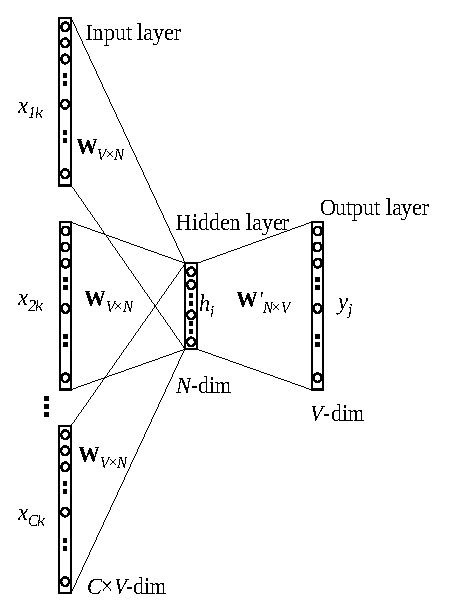
\includegraphics[width=.4\textwidth]{CBOW.pdf}%
    \caption{CBOW model with \(C\) words in the context.}
  \end{figure}
\end{frame}

\begin{frame}{Continuous Bag-of-Words Model}{Definition}
  \begin{itemize}
  \item The input consists of one\-/hot encoded words,
    \(\vec{x}_1, \ldots, \vec{x}_C\).
  \item The input \(\to\) hidden and hidden \(\to\) output weights are
    represented by \(\mat{W}\) and \(\mat{W}'\) respectively.  The
    rows of \(\mat{W}\) (denoted \(\vec{v}_w\)) and the columns of
    \(\mat{W}'\) (denoted \(\vec{v}'_w\)), give the
    \alert{\(N\)\=/dimensional input} and \alert{output
      representations} of a word \(w\).
  \item The hidden layer is \emph{linear} and computes an average
    \[
      \vec{h} \coloneqq \frac{(\sum_{c = 1}^{C} \vec{x}_c) \mat{W}}{C}
      = \frac{\sum_{c = 1}^{C} \vec{v}_{w^{\ins}_c}}{C}\text.
    \]
  \item The output layer is a softmax panel outputting a multinomial
    distribution over the vocabulary.
  \end{itemize}
\end{frame}

\begin{frame}{Continuous Bag-of-Words Model}{Update Equations}
  As usual with softmax, the cross\-/entropy loss function is used,
  \begin{equation}\label{eq:cross-entropy}
    \begin{aligned}
      E &\coloneqq -\log p(w^{\outs} \mid w^{\ins}_1, \ldots, w^{\ins}_C)\\
      &= -\vec{v}_{w^{\outs}}^{\prime\trans} \vec{h} + \log \sum_{v =
        1}^{V} \exp(\vec{v}_{w_v}^{\prime\trans} \vec{h})\text.
    \end{aligned}
  \end{equation}
  By taking the corresponding derivatives of~\eqref{eq:cross-entropy},
  we arrive at the update equations:
  \begin{equation}\label{eq:update-equations}
    \begin{aligned}
      \vec{v}'_{w_v}&\coloneqq \vec{v}'_{w_v} - \eta e_v \vec{h}\\
      \vec{v}_{w^{\ins}_c} &\coloneqq \vec{v}_{w^{\ins}_c} -
      \frac{\eta}{C} \frac{\partial E}{\partial \vec{h}}\text.
    \end{aligned}
  \end{equation}
\end{frame}

\begin{frame}{Continuous Bag-of-Words Model}{Understanding the Update
    Equations}
  The derivatives in~\eqref{eq:update-equations} can be computed using
  backpropagation:
  \begin{align*}
    e_v &= \text{prediction error for word}\ v\text,\\
    \frac{\partial E}{\partial h_i} &= \sum\limits_{v = 1}^{V} e_v w'_{i v}\text.
  \end{align*}
  Intuitively,
  \begin{itemize}
  \item If we overestimate (resp.\ underestimate) the probability for word
    \(w_v\), we subtract from (resp.\ add to) \(\vec{v}'_{w^{\outs}}\) a portion of
    the input \(\implies\) \(\vec{v}'_{w^{\outs}}\) becomes closer to the averaged
    input vectors.
  \item Since \(\partial E / {\partial \vec{h}}\) is the sum of all
    output vectors weighted by their prediction
    errors,~\eqref{eq:update-equations} can be seen as distributing a
    portion of every output vector to each of the \(C\) input vectors.
  \end{itemize}
\end{frame}

\begin{frame}{Skip-Gram Model}{Illustration}
  \begin{figure}
    \centering
    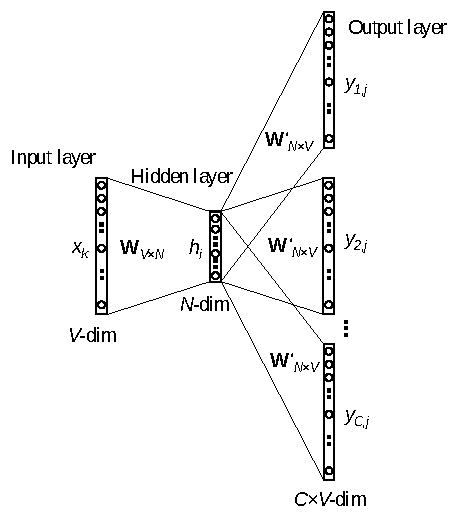
\includegraphics[width=.4\textwidth]{Skip-Gram.pdf}
    \caption{Skip-gram model for predicting \(C\) context words.}
  \end{figure}
\end{frame}

\begin{frame}{Skip-Gram Model}{Definition}
  \begin{itemize}
  \item The input consists of a one\-/hot encoded word, \(\vec{x}\),
    with \(x_k = 1\) and \(x_i = 0\) for all \(i \ne k\).
  \item The weights encode the same information as in the CBOW model.
  \item The hidden layer simply copies the row of the matrix
    \(\mat{W}\) associated with the input word \(w^{\ins}\):
    \[
      \vec{h} = \mat{W}_{(k, \cdot)} \eqqcolon
      \vec{v}_{w^{\ins}}\text.
    \]
  \item The output layer consists of \(C\) softmax panels, and outputs
    \(C\) multinomial distributions over the vocabulary.
  \end{itemize}
\end{frame}

\begin{frame}{Skip-Gram Model}{Update Equations}
  Again, we use the cross\-/entropy loss function.  Note that care
  must be taken as we are now dealing with \(C\) multinomial
  distributions rather than just one.
  \begin{align*}
    E &\coloneqq -\log p(w^{\outs}_1, \ldots, w^{\outs}_C \mid w^{\ins})\\
      &= -\sum_{c = 1}^{C} \vec{v}_{w^{\outs}_c}^{\prime\trans} \vec{h} +
        C \log \sum_{v = 1}^{V} \exp(\vec{v}_{w_v}^{\prime\trans} \vec{h})\text.
  \end{align*}
  The equations are identical as in the CBOW model, except the
  prediction errors must be summed across all \(C\) softmax panels.
  \[
    e_v = \sum_{c = 1}^{C}(\text{prediction error of the}\
    c\text{\=/th softmax panel for word }v)\text.
  \]
\end{frame}

\begin{frame}{Issues With the CBOW and Skip-Gram Models}
  \begin{itemize}
  \item Both models are very similar in their nature and have a same
    intuitive interpretation.
  \item Due to the smoothing, CBOW is recommended for small datasets;
    while skip-gram is able to learn better representations give
    sufficient data (\enquote{there is no better regulizer than a
      large dataset}).
  \item Unfortunately, both are very hard to train.
  \end{itemize}
  We tried to avoid the vast size of the vocabulary as hard as
  possible, however,~\eqref{eq:update-equations} performs
  \(\BigOh(V)\) weight updates for both the CBOW and skip\-/gram
  models.  To ameliorate this and make learning practical, we will
  look at:
  \begin{itemize}
  \item hierarchical softmax; and
  \item negative sampling.
  \end{itemize}
\end{frame}

\subsection{Making Learning by Prediction Practical}

\begin{frame}{Hierarchical Softmax}
  The hierarchical softmax uses a binary tree to represent the
  vocabulary.  There are \(V\) leaves, one for each word; and
  \(V - 1\) inner units.
  \begin{figure}
    \centering
    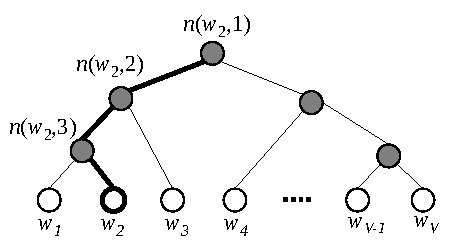
\includegraphics[width=.5\textwidth]{Hierarchical_Softmax.pdf}
    \caption{Example hierarchical softmax with path to \(w_2\).}
  \end{figure}  
\end{frame}

\begin{frame}{Hierarchical Softmax}{Details}
  \begin{itemize}
  \item There is no output vector representation\--- each of the
    \(V - 1\) inner units has an output vector \(\vec{v}_{n(w, j)}\).
  \item The probability of a word being the output word is
    \[
      \Pr(w = w^{\outs}) = \prod_{j = 1}^{\mathclap{L(w) - 1}}
      \sigma(\Iverson{n(w, j + 1) = \Left(n(w, j))}
      \vec{v}^{\prime\trans}_{n(w, j)} \vec{h})\text,
    \]
    where \(L(w)\) is the length of the path to word \(w\),
    \(\Left(n(w, j))\) is the left child of the inner unit
    \(n(w, j)\), \(\sigma\) is the sigmoid function, and
    \[
      \Iverson{p} =
      \begin{cases}
        1 & \text{if}\ p\ \text{is true}\\
        -1 & \text{otherwise.}
      \end{cases}
    \]
  \end{itemize}
\end{frame}

\begin{frame}{Hierarchical Softmax}{Update Equations}
  By backtracing the path from the leaves to the root, one obtains the
  update equations for the inner nodes:
  \[
    \vec{v}'_{n(w, j)} \coloneqq
    \vec{v}'_{n(w, j)} - \eta
    (\sigma(\vec{v}^{\prime\trans}_{n(w, j)} \vec{h}) - t_{n(w, j)})
    \vec{h}\text,
  \]
  where \(t_{n(w, j)}\) denotes the \enquote{ground truth} at level
  \(j\) (\enquote{left} or \enquote{right}).

  The derivative of the error with respect to the hidden layer can be
  found as
  \[
    \frac{\partial E}{\partial \vec{h}} = \sum_{j = 1}^{L(w) - 1}
    (\sigma(\vec{v}^{\prime\trans}_{n(w, j)} \vec{h}) - t_j)
    \vec{v}'_{n(w, j)}\text.
  \]
\end{frame}

\begin{frame}{Hierarchical softmax}{Bottom line}
  \begin{itemize}
  \item Hierarchical softmax can be applied to both the CBOW and
    skip\-/gram models.
  \item For CBOW, one can plug in the equations directly.  For
    skip\-/gram, we need to iterate over the entire context that is
    being predicted.
  \item Computational complexity is reduced from \(\BigOh(V)\) to
    \(\BigOh(\log V)\).
  \item Number of parameters remains roughly the same.
  \end{itemize}

  \structure{Can we do even better?}  Turns out, if some heuristic
  assumptions are satisfied, we can.
\end{frame}

\begin{frame}{Negative Sampling}{Assumption}
  The idea is very straightforward: instead of updating all output
  vectors, update only a sample of them.
  \begin{assumption}[Negative Sampling]
    In order to learn the context, it is enough to update only the
    output word (\enquote{ground truth}) along with a few words as
    negative samples.
  \end{assumption}
  The negative samples are drawn from a noise distribution
  \(p^{\negs}(w)\) which is determined empirically.  \Verb+word2vec+
  uses the unigram distribution raised to the power of \(3 / {4}\).
\end{frame}

\begin{frame}{Negative Sampling}{Loss Function and Error Derivatives}
  For further heuristics, negative sampling does not use a loss
  function that produces a well\-/defined posterior multinomial
  distribution.
  \[
    E = -\log \sigma(\vec{v}^{\prime\trans}_{w^{\outs}} \vec{h}) -
    \sum_{\mathclap{w^{\negs} \in \mat{W}^{\negs}}} \log
    \sigma(-\vec{v}^{\prime\trans}_{w^{\negs}} \vec{h})\text{,}
  \]
  where \(\mat{W}^{\negs}\) is a set of negative samples.  This
  results in updates very similar to the hierarchical softmax.
  Writing
  \(\mathcal{W} \coloneqq \{w^{\outs}\} \cup \mat{W}^{\negs}\),
  \begin{align*}
    \vec{v}'_{w_j}%
    &
      \coloneqq \vec{v}'_{w_j} -
      \eta (\sigma(\vec{v}^{\prime\trans}_{w_j} \vec{h}) - t_j) \vec{h}\\
    \frac{\partial E}{\partial \vec{h}}%
    &=
      \sum_{w_j \in \mathcal{W}}
      \frac{\partial E}{\partial \vec{v}^{\prime\trans}_{w_j} \vec{h}}
      \frac{\partial \vec{v}^{\prime\trans}_{w_j} \vec{h}}{\partial \vec{h}}
      =
      \sum_{w_j \in \mathcal{W}}
      (\sigma(\vec{v}^{\prime\trans}_{w_j} \vec{h}) - t_j) \vec{v}'_{w_j}\text,
  \end{align*}
  for all \(w_j \in \mathcal{W}\); where
  \(t_j \coloneqq \mathbb{1}\{w_j = w^{\outs}\}\).
\end{frame}

\begin{frame}{Further Improvements}{Subsampling}
  In order to counter the imbalance between rare and frequent words,
  \Verb+word2vec+ uses subsampling.  Namely, each word in the training
  set is discarded with probability
  \[
    1 - \sqrt{\frac{d}{f(w_j)}}\text,
  \]
  where \(f(w_j)\) is the frequency of the word \(w_j\) and \(d\) is
  the discard threshold, typically around \num{e-5}.
\end{frame}

\section{Reasoning With Word Vectors}

\begin{frame}{Country--Capital City Relationships}
  \begin{figure}
    \centering
    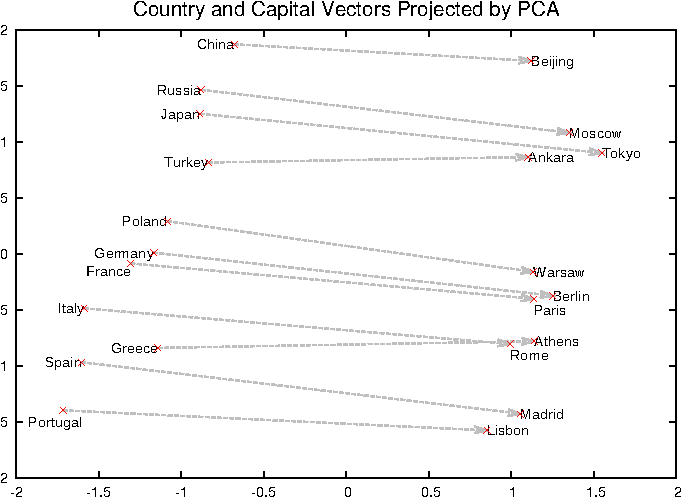
\includegraphics[width=.75\textwidth]{Country--Capital_Vectors.pdf}
    \caption{Country\--capital city relationships projected with PCA.}
  \end{figure}  
\end{frame}

\begin{frame}{Phrase Representations}
  The aforementioned models are not restricted only to words\--- they
  can use phrases and other constructs just as well.
  \begin{table}
    \centering
    \caption{Phrase analogy with \num{e-5} subsampling.}
    \begin{tabular}{c c c}
      \toprule
      Phrase & NEG & HS\\
      \midrule
      Vasco de Gamma & Lingsugur & Italian explorer\\
      Lake Baikal & Great Rift Valley & Aral Sea\\
      Alan Bean & Rebbeca Naomi & moonwalker\\
      Ionian Sea & Ruegen & Ionian Islands\\
      chess master & chess grandmaster & Garry Kasparov\\
      \bottomrule
    \end{tabular}
  \end{table}
\end{frame}

\begin{frame}{Additive Compositionality}
  Interestingly, element\-/wise addition yields meaningful
  combinations, too.  This property can be explained by looking at the
  training objective: the vectors are related logarithmically to the
  probabilities computed by the output layer, so the sum of two word
  vectors is related to the product of the two context distributions.
  \begin{table}
    \centering
    \caption{Additive compositionality showing the \num{4} closest vectors.}
    \resizebox{\linewidth}{!}{%
      \begin{tabular}{c c c c c}
        \toprule
        Czech + currency & Vietnam + capital & German + airlines & Russian + river%
        & French + actress\\
        \midrule
        Koruna & Hanoi & airline Lufthansa & Moscow & Juliette Binoche\\
        Czech crown & Ho Chi Minh City & carrier Lufthansa & Volga River%
        & Vanessa Paradis\\
        Polish zolty & Viet Nam & flag carrier Lufthansa & upriver%
        & Charlotte Gainsbourg\\
        CTK & Vietnamese & Lufthansa & Russia & Cecile De\\
        \bottomrule
      \end{tabular}%
    }
  \end{table}
\end{frame}

\end{document}

%%% Local Variables:
%%% mode: latex
%%% TeX-command-extra-options: "-shell-escape"
%%% TeX-engine: luatex
%%% TeX-master: t
%%% End: